%%%%%%%%%%%%%%%%%%%%%%%%%%%%%%%%%%%%%%%%%%%%%%%%%%%%%%%%%%%%%%%%%%%%%%%%%%%
% Juan Manuel Perez Rua
%%%%%%%%%%%%%%%%%%%%%%%%%%%%%%%%%%%%%%%%%%%%%%%%%%%%%%%%%%%%%%%%%%%%%%%%%%%

\section{Background regions tracking and segmentation}
\label{sec:segm}
The algorithm proposed in \cite{c18}, offers a good deal in terms of
background-foreground separation from user interaction. A technique like this, however,
performs very well in still images, but it may not be well adapted for sequential videos. 
Extensions to this method, like the GrabCut algorithm (\cite{c14}), work by implementing an iterative graph-cut based 
minimization to separate regions according to appearance information from a loosely drawn rectangle around the object, and small user-interaction-based hints. 
Given the tracker state for every frame, the minimization procedure of the methods in \cite{c18} and \cite{c14} could be extended to video. However, 
a lot of details in the segmentation contour may be lose if no fine hints are given.
These hints usually depend on on-the-fly supervised methods. However, this need could be minimized in videos, given the extra information that offers the flow of the sequence.
Some authors had approached the graph-cut based segmentation techniques in sequential
videos to propagate a consistent segmentation \cite{c15}. However, some more work on reducing user interaction given the extra flow-like information
that video sequences offer is still needed.
We propose to combine the presented superpixel flow as an automatic initialization method for the desired segmentation method.
 
The main idea to perform object segmentation consist in tracking (or more exactly, matching) superpixels that are labelled as background, thanks to an object tracker initialization. Thus, the superpixels that are initially outside the tracker region of interest, 
can be propagated through the sequence, and if they fall into the window on a subsequent frame, they
can be safely labelled as background (Fig.  \ref{figurelabel_entering}). \\

   \begin{figure}[thpb]
      \centering
      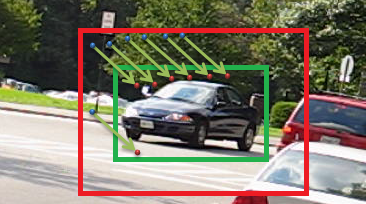
\includegraphics[height=0.25\textheight]{../images/tracking_points.png}
      \caption{Example image of points entering a tracking region (green) due to object motion in a video sequence.}
      \label{figurelabel_entering}
   \end{figure}
\setlength{\belowcaptionskip}{-10pt}

To save computational power, the tracked superpixels are 
limited to the ones that fall inside a control region (red box in the Fig.  \ref{figurelabel_entering}). Usually, after several frames, 
the labeled superpixels will almost completely cover the unwanted areas in a dinamyc scene. We call this process background segments tracking.  The Fig. \ref{figurelabel_spflow} shows this idea in a real scenario. From left to right, initially the superpixels with 
elements outside the bounding box are labeled as background (green), then, as the sequence changes, the labeled superpixels flow inside the window, giving hints for the model initialization in the background-foreground separation algorithm. 
At this point, some generic segmentation technique can be connected to the pipeline to refine the segmentation (e.g. region growing). We prefer, however graph based segmentation methods (\cite{c18}\cite{c15}) because the usual user interaction can be replaced by the tracked background regions.
%Having several labeled superpixels can reduce widely or totally the necessity for user interaction in subsequent frames in %comparison with other segmentation techniques. Thus, to perform object segmentation in a full video sequence, the required
%user interaction would only be the initial bounding box. Moreover, a fully automatic approach can be
%obtained if a reliable object detector is available.

   \begin{figure}[thpb]
      \centering
      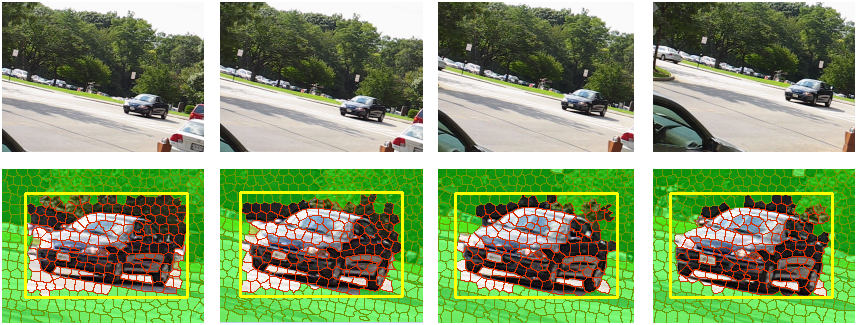
\includegraphics[width=1\textwidth]{../images/suppixflow2.png}
      \caption{Background segments automatic labeling and propagation, the flow goes from left to right.}
      \label{figurelabel_spflow}
   \end{figure}

\subsection{Segmentation results}

Fig. \ref{figurelabel_walking} shows the results for an image sequence where the interest object is the head of a person.
The head tracker and the superpixel flow provide information for better background-foreground separation. The
background-foreground models are updated as the frames go on, giving more robustness for sequential
propagation of the segmentation. The method is tested in the Walking Couple sequence, by allowing only a small amount of iterations in the
graph based segmentation. Observe how the contour in the man's head is correctly delineated when
another person's head occludes part of it. In this case, the superpixels that belong to the woman’s face
were correctly propagated and thus, labeled as background. \\
   \begin{figure}[thpb]
      \centering
      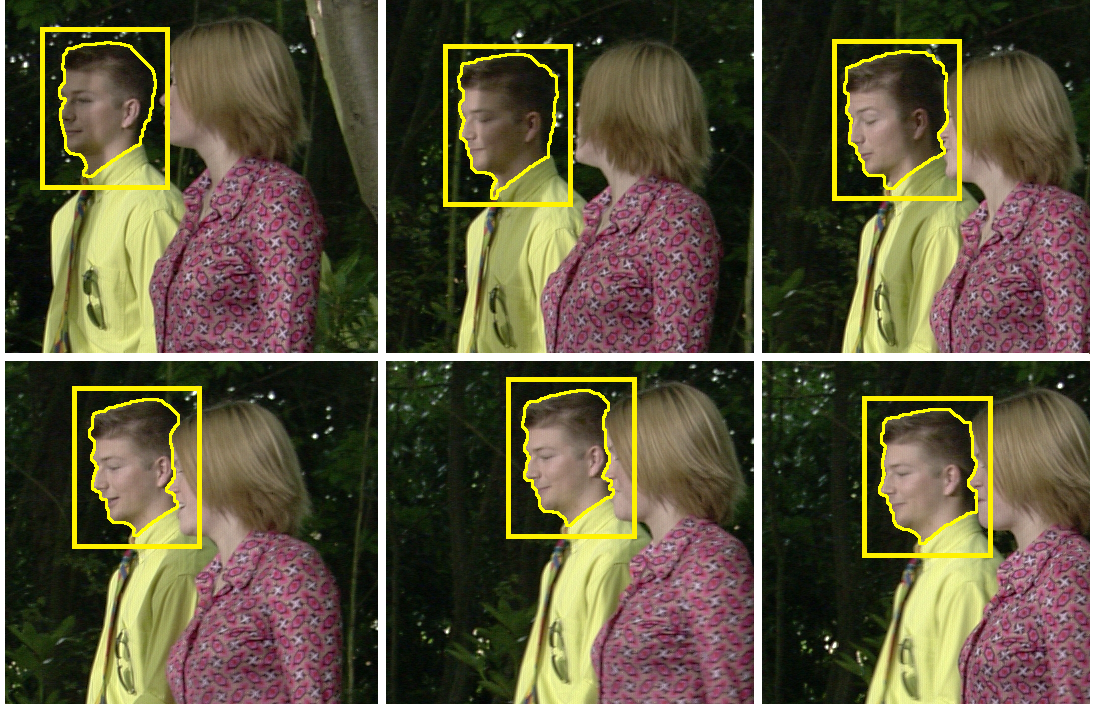
\includegraphics[width=1.0\textwidth]{../images/Sequence2.png}
      \caption{Segmentation through the sequence “Walking
	       Couple” (Yellow contour) initialized in the man’s head. The yellow box correspond to the tracker output.
	        The labeled background superpixel are not shown for clarity.}
      \label{figurelabel_walking}
   \end{figure}

In order to understand the effect of including superpixel propagation in a video sequence for object
segmentation, some results are shown in the Fig. \ref{figurelabel_comp}. For these experiments only one iteration is
allowed in the graph-cut based methods. The top row frames (Fig. \ref{figurelabel_comp}) were initialized only with the tracker, 
and the bottom row was initialized with the superpixel tracking technique. 
Observe that in general, the contour delineated is usually better in terms of precision and
stability for the later one.
   \begin{figure}[thpb]
      \centering
      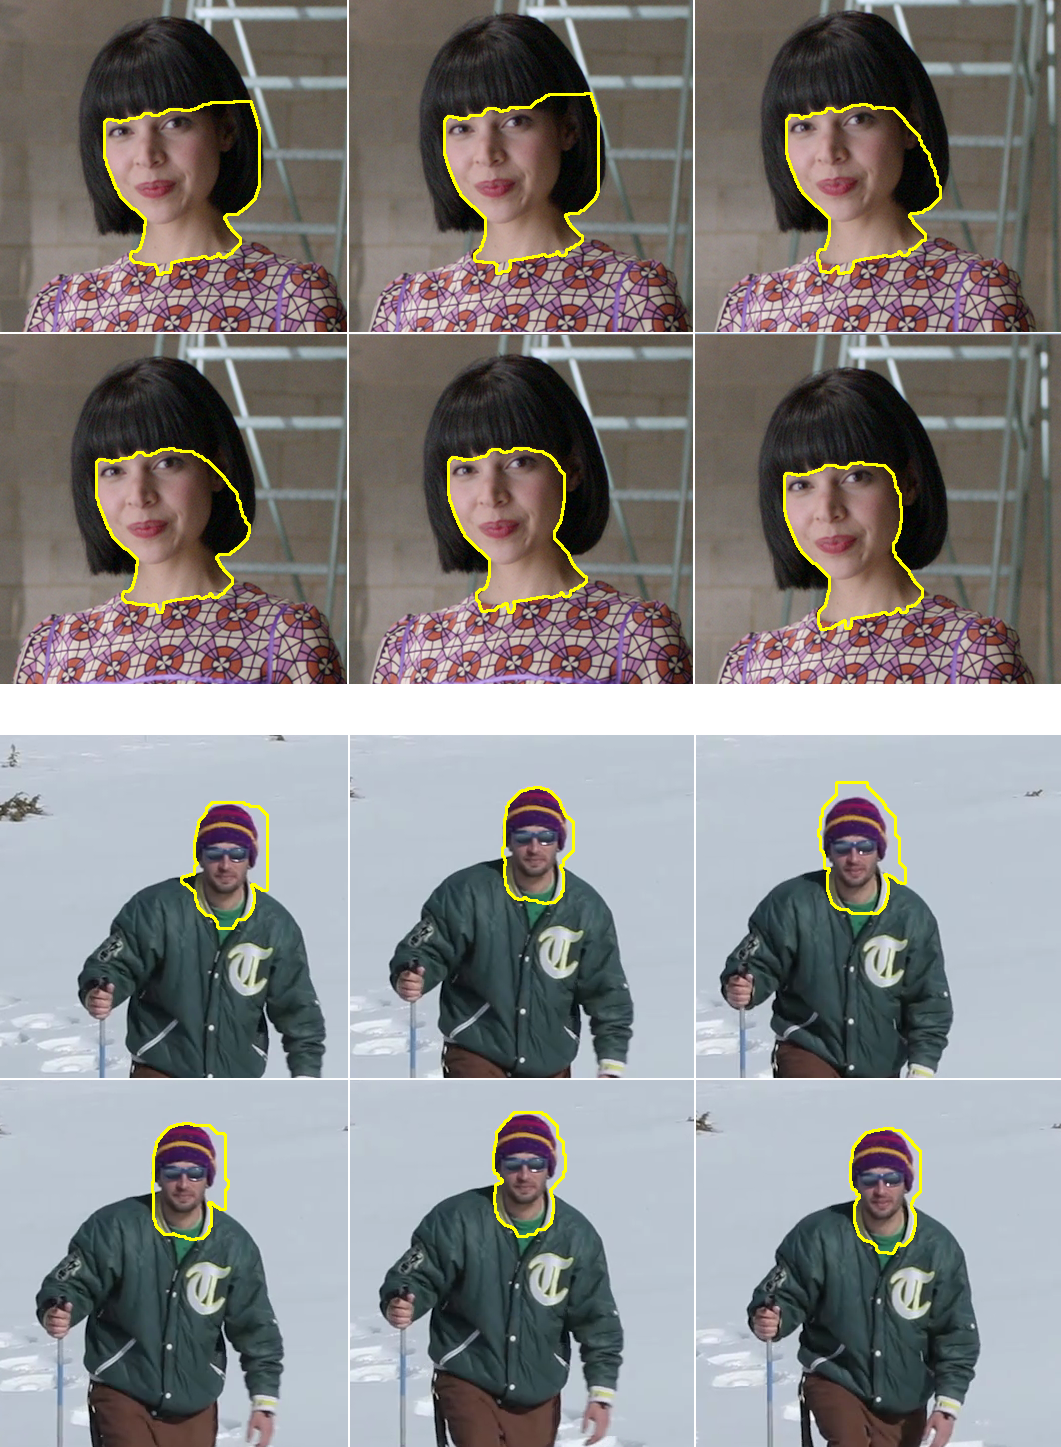
\includegraphics[width=0.9\textwidth]{../images/Compare.png}
      \caption{Face segmentation in the “Amelie Retro” and the
	      “Snow shoes” sequences in three different frames. For each
	       group, the Top Row: One-iteration window-based graph-cuts;
	       and the Bottom Row: One-iteration graph-cuts initialized with superpixel tracking.}
      \label{figurelabel_comp}
   \end{figure}
